\chapter{Self-testing}
\lhead{\emph{Self-testing}}
\label{sec:self-testing}

Self-testing aims to certify properties of unknown quantum devices, only by interacting classically with these, i.e.\ by passing classical input strings to devices and receiving classical outputs, for instance a binary string. Ideally, we want to make a minimal number of assumptions about the devices themselves, largely treating them as black boxes\footnote{Self-testing schemes that do not require assumptions about the underlying mechanics of the devices, and consider only the input-correlations they generate, are called ``device-independent".}. This is useful for certifying the behaviour of untrusted or noisy quantum devices, even in an adversarial scenario, and for the most part does not require the experimenter to have knowledge about the exact inner workings of the devices. 
More concretely, many quantum key distribtion (QKD) protocols for quantum cryptography, such as Ekert91 \cite{Ekert91}, require the generation of a large number of maximally entangled states. To ensure information-theoretic security, one has to confirm the quality of the entanglement source used. Self-testing provides a means of doing this.

A self-testing protocol is essentially a correlation experiment, as introduced in Section \ref{sec:correxp}, that allows us to make powerful inferences about the internal workings of the devices. The following example will clarify the concept. We will still assume measurements to be sharp for now:

Consider the CHSH correlation experiment, as introduced in Section \ref{sec:bell}, with two space-like separated systems, $\mathcal{A}$ and $\mathcal{B}$, as well as two experimenters that can perform local measurements. Assuming no-signalling, i.e.\ that local measurements on $\mathcal{A}$ do not disturb the outcome statistics of local measurements on $\mathcal{B}$, remote measurements are compatible according to Defintion \ref{def:compat}. Recall that the CHSH correlation experiment is a test for violations of the inequality
\begin{align*}
    \frac{1}{4}(\; & p(x=y\vert A_1,B_1)+p(x=y\vert A_2,B_1)\\ +\thinspace&p(x=y\vert A_2,B_2)+p(x\neq y \vert A_1,B_2) \;)\leq \frac{3}{4}
\end{align*}
The exclusivity graph of the CHSH correlation experiment can be seen in Figure \ref{fig:chshexcl}; the equal weighting $\frac{1}{4}$ each vertex receives is omitted for readability. 

\begin{figure}
    \centering
    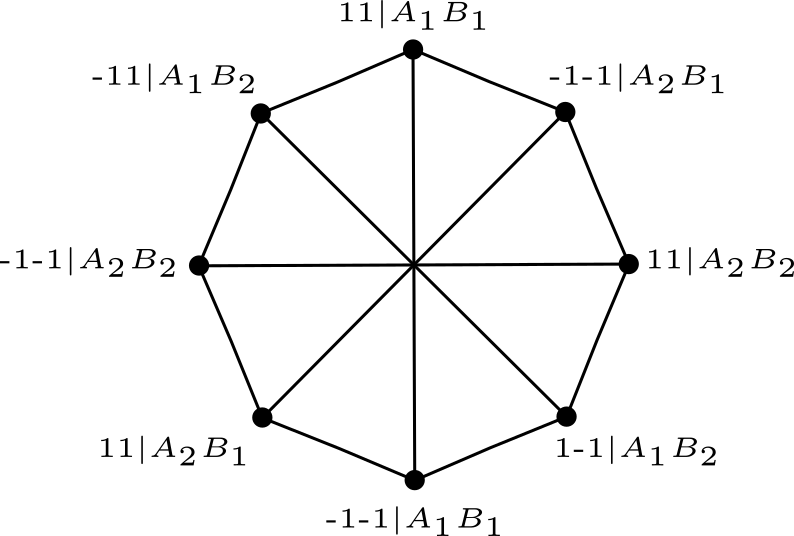
\includegraphics[width=0.6\textwidth]{images/chshexcl.png}
    \caption{Exclusivity graph for the CHSH correlations experiment, see Section \ref{sec:bell}. Like in Section \ref{sec:bell}, the outcomes of local measurements are labelled $\pm 1$. Vertices correspond to measurement events, exclusive measurement events are represented as adjacent.}
    \label{fig:chshexcl}
\end{figure}

The Lovász number of the CHSH exclusivity graph corresponds to the Tsirelson bound $B_q = \frac{1}{2}(1+\frac{1}{\sqrt{2}})$. Thus, the Lovász bound is tight and the measurements \ref{eqn:chshmnts}, together with the maximally entangled EPR state, produce a maximal violation of the CHSH inequality \ref{eqn:chshineq}. 

In fact, due to space-like separation, the Lovász bound is a tight upper bound that all correlations compatible with QM have to obey, even if we allow for general POVM measurements. This follows from the Naimark dilation theorem \cite{Watrous2018}. Informally, we can extend every non-projective quantum measurement $\{M_i\}_i$ acting on the system $\mathcal{A}$ to a projective measurement $\{\Pi_i^{\mathcal{A}}\}_i$ that acts on a composite system $(\thinspace\mathcal{A}+\text{ancilla}\thinspace)$, where the ancillary system is prepared in some well-defined state $\ket{0}\bra{0}$. The extended projectors acting on the composite system $(\thinspace\mathcal{A}+\text{ancilla}\thinspace)$ produce the same output correlations as the unsharp measurements acting on the single system $\mathcal{A}$. The same can be said about local measurements on subsystem $\mathcal{B}$. Now, due to space-like separation, the projectors $\Pi_i^{\mathcal{A}}\otimes \Pi_j^{\mathcal{B}}$ corresponding to exclusive measurement events commute. As such, we can follow the same line of reasoning as in Section \ref{sec:complicationscont} to argue that the maximal violation of the CHSH inequalitiy, even with access to unsharp measurements is given by the Tsirelson bound. As we saw in Section \ref{sec:complicationscont}, the same considerations do not apply to contextuality scenarios involving compatible measurements on a single system. While we can extend the individual measurements to projective measurements by adding an ancilliary system, thereby associating with each measurement event a projector, we have no grounds to assume that the projectors associated with exclusive measurement are orthogonal. Take for instance the KCBS correlation experiment with exclusivity graph Figure \ref{fig:kcbsexclusivity}. Measurements 1,2 and 2,3 are compatible, however not all three are jointly measurable. We can assume the Naimark projectors associated with the measurement events $0,1\thinspace\vert\thinspace 1,2$ and $0,0\thinspace\vert\thinspace 1,2$ to be orthogonal, because they correspond to distinct outcomes of a single joint measurements. This does not hold for the exclusive measurement events of the KCBS exclusivity graph: $0,1\thinspace\vert\thinspace 1,2$ and $0,1\thinspace\vert\thinspace 2,3$ can not be distinct outcomes of a single joint measurement, as the measurements $1,2,3$ are not even pairwise compatible.

Back to the CHSH correlation experiment: A violation of the CHSH inequality implies that the observed correlations are not compatible with a classical description of the form \ref{eqn:lhvm}, but require quantum resources, in particular entanglement, to generate. What is remarkable about, but not unique to the CHSH Bell inequality\footnote{Other Bell inequalities may self-test different reference experiments.}, is that the quantum model presented in \ref{eqn:chshmnts}, leading to a maximal violation of the inequality, i.e.\ corresponding to the extremal point $\Vec{v}_{max}\in\mathcal{Q}$ of the set of quantum correlations, see Figure \ref{fig:selftestingcorr}, is ``essentially unique". By this we mean that the only quantum model $\ket{\Psi}$, $\{\Pi_i\}_i$ predicting a maximal violation of the CHSH inequality is \ref{eqn:chshmnts}, modulo trivial changes to the reference experiment which we will specify shortly. A comprehensive proof is given in \cite{Supic2020}.
Thus, by interacting only classically with our preparation and measurement devices, we can characterize the quantum state and measurements our devices implement. We can only hope to self-test extremal correlations, as other correlations $\Vec{v}\in\mathcal{Q}$ correspond to a non-unique convex combination of distinct extremal correlations. 

It is apparent that we can never certify exact states and measurements, as we will always be blind to a number of trivial degrees of freedom. For instance, we cannot tell if there are any additional ancilliary systems, $\mathcal{A'}$, $\mathcal{B'}$, prepared in some joint state $\rho_{\mathcal{A'B'}}$, in the remote labs that we are not probing:
\begin{align*}
    & \ket{\Psi}_\mathcal{AB}\thinspace,\thinspace && A_{1} = \sigma_{z,\mathcal{A}}\otimes\mathbb{1}_{\mathcal{B}}\thinspace,\thinspace \dots \\
    \equiv\; & \ket{\Psi}\bra{\Psi}_{\mathcal{AB}}\otimes\rho_{\mathcal{A'B'}}\thinspace,\thinspace && A_1 = \sigma_{z,\mathcal{A}}\otimes\mathbb{1}_{\mathcal{A'BB'}}\thinspace,\thinspace\dots\; .
\end{align*}
Furthermore, we can never detect local unitaries $U=U_\mathcal{AA'}\otimes U_\mathcal{BB'}$, i.e.\ local basis changes:
\begin{align*}
    & \ket{\Psi}\bra{\Psi}_{\mathcal{AB}}\thinspace\otimes\thinspace\rho_{\mathcal{A'B'}}\thinspace,\thinspace && A_1 = \sigma_{z,\mathcal{A}}\thinspace\otimes\thinspace\mathbb{1}_{\mathcal{A'BB'}}\thinspace,\thinspace\dots \\ 
    \equiv\;  U(& \ket{\Psi}\bra{\Psi}_{\mathcal{A,B}}\thinspace\otimes\thinspace\rho_{\mathcal{A'B'}})U^{\dag}\thinspace,\thinspace && A_1 = U_{\mathcal{AA'}}(\sigma_{z,\mathcal{A}}\thinspace\otimes\thinspace\mathbb{1}_{\mathcal{A'BB'}})U_{\mathcal{AA'}}^{\dag}\thinspace,\thinspace\dots\; .
\end{align*}

According to Stinespring's Dilation Theorem \cite{Watrous2018}, these trivial degrees of freedom can account for arbitrary local isometries $\mathcal{A}\rightarrow\mathcal{AA'}$, $\mathcal{B}\rightarrow\mathcal{BB'}$. Furthermore, the previous two examples suggest that in order to define a sensible notion of self-testing, we must first define some notion of equivalence for quantum models. We then aim to construct self-testing protocols that single out a unique quantum model, modulo this notion of equivalence. This notion of equivalence should account for some trivial degrees of freedom, like the ones above, but should also not be too broad, in order for self-testing to be a powerful property of select correlation experiments. Ideally, the equivalence of quantum realizations should have an operational meaning. The following definition applies to Bell-type correlation experiments and does justice to these three criteria.

\begin{definition}[\cite{McKague2011}]
\label{def:equivexp}
A quantum experiment involving $\ket{\Psi'}_{\mathcal{A'B'P}}$ and local measurements $\{{P'}^{\thinspace a}_x\}_x$, $\{{Q'}^{\thinspace b}_y\}_y$, where $\ket{\Psi'}_{\mathcal{A'B'P}}$ is an arbitrary purification and ${P'}^{\thinspace a}_x$ is the positive semi-definite operator corresponding to the outcome $x$ of the local measurement $a$ on system $\mathcal{A}$, is \emph{equivalent} to a reference experiment $\ket{\Psi}_{\mathcal{AB}}, \{P_x^a\}_x$, $\{Q_y^b\}_y$, if there exists a local isometry $\Phi=\Phi_{\mathcal{A}}\otimes\Phi_{\mathcal{B}}$, $\Phi_{\mathcal{A/B}}\colon\mathcal{H}_{\mathcal{A'/B'}}\rightarrow\mathcal{H}_{\mathcal{A'/B'}}\otimes\mathcal{H}_{\mathcal{A/B}}$, such that
\begin{align*}
    (\Phi\otimes\mathbb{1}_{\mathcal{P}})\ket{\Psi'}_{\mathcal{A'B'P}} & =\ket{\text{junk}}_\mathcal{{A'B'P}}\otimes\ket{\Psi}_{\mathcal{AB}} \\[0.7em]
    (\Phi\otimes\mathbb{1}_{\mathcal{P}})({P'}^{\thinspace a}_x\otimes {Q'}^{\thinspace b}_y)\ket{\Psi'}_{\mathcal{A'B'P}} & =\ket{\text{junk}}_{\mathcal{A'B'P}}\otimes(P^a_x\otimes Q^b_y)\ket{\Psi}_{\mathcal{AB}} \thinspace .
\end{align*}
\end{definition}

Operationally, this means that a physical experiment is equivalent to some reference experiment if by means of local operations alone\footnote{Note that the two experimenters can realize an arbitrary local isometry $\Phi=\Phi_{\mathcal{A}}\otimes\Phi_{\mathcal{B}}$ by preparing ancilliary systems in some well-defined state $\ket{00}$ and subsequently applying local unitary operations.}, one can recover the reference experiment, up to some ``junk". In particular, the experimenters can for instance extract the reference state, i.e.\ the maximally entangled EPR state for the CHSH correlation experiment, to their ancilliary systems, by means of local operations alone. As local operations cannot generate entanglement, their initial state must have been maximally entangled. Note that the notion of equivalence, as defined in Definition \ref{def:equivexp}, is not an equivalence relation, as it fails to be symmetric \cite{McKague2011}.  While the experimenters can extract the reference state to ancilliary systems using only local operations, if they have access to an equivalent experiment, the converse direction must not hold: Consider the reference CHSH experiment \ref{eqn:chshmnts} producing a maximal violation of the CHSH inequality \ref{eqn:chshineq}. Further, consider the equivalent quantum experiment where both experimenters control an additional ancilliary system and both ancillae are prepared in an entangled state. While this extended experiment is equivalent to the reference experiment, the converse does not hold, as we cannot create entanglement by local operations alone.

Definition \ref{def:equivexp} accounts for all of the following statistics-preserving trivial degrees of freedom, as presented in \cite{McKague2011}:
\begin{enumerate}
    \item Local changes of basis
    \item adding ancillae to the physical systems, prepared in any joint state (measurements do not act on these)
    \item changing the action of an observable outside the support of the state
    \item locally embedding the state and operators into a larger (or smaller) Hilbert space
\end{enumerate}

\begin{claim}[\cite{McKague2011}]
Any finite number of changes 1-4 transforms a quantum experiment into an equivalent quantum experiment like in Definition \ref{def:equivexp}. Furthermore, any quantum experiment equivalent to some reference experiment can be constructed from that reference experiment by applying  a finite number of changes 1-4.
\end{claim}

Let us constrast self-testing via Bell inequalities with self-testing via KS non-contextuality inequalities. Section \ref{sec:contselftesting} will examine in detail a self-testing protocol based on the class of odd $n$-cycle KS non-contextuality inequalities \cite{Bharti2019}. Importantly, without space-like separated subsystems, we have to give up device-independence: While relaxing the assumption of space-like separation means that we no longer require the device to be split up among remote subsystems, or that it can generate a large number of entangled states, we can no longer make use of quantum non-locality to certify that the correlations were not simulated by some pre-programmed classical computer \cite{Supic2020}. In principle, we can never discard this possibility without imposing additional assumptions about the devices. In Section \ref{sec:memoryass}, we examine how bounding the information carrying capacity or memory of the device can be helpful in this regard. Additionally, the CSW framework in Section \ref{sec:csw}, which gives us non-trivial constraints on the set of valid quantum models, which we will be use in the self-testing proof, requires assumptions about operator compatibility and sharpness. This is illustrated in Figure \ref{fig:selftesting}. Since contextuality scenarios no longer require remote subsystems, we need to amend our notion of ``equivalence" for quantum experiments, see Definition \ref{def:equivexp}, accordingly. We will come back to this in Section \ref{sec:contselftesting}, but already note that contextuality-based self-testing protocols aim to single out a quantum realization, up to a \textbf{global} isometry.

Finally, self-testing results should be robust to noise. Informally, this means that a near-optimal violation of the Bell or KS non-contextuality inequality should imply that all compatible quantum models are, up to equivalence, ``close" to the reference quantum experiment. The self-testing protocol we will examine in Section \ref{sec:contselftesting} is robust, see Theorem \ref{thm:contselftesting}.

\begin{figure}
    \centering
    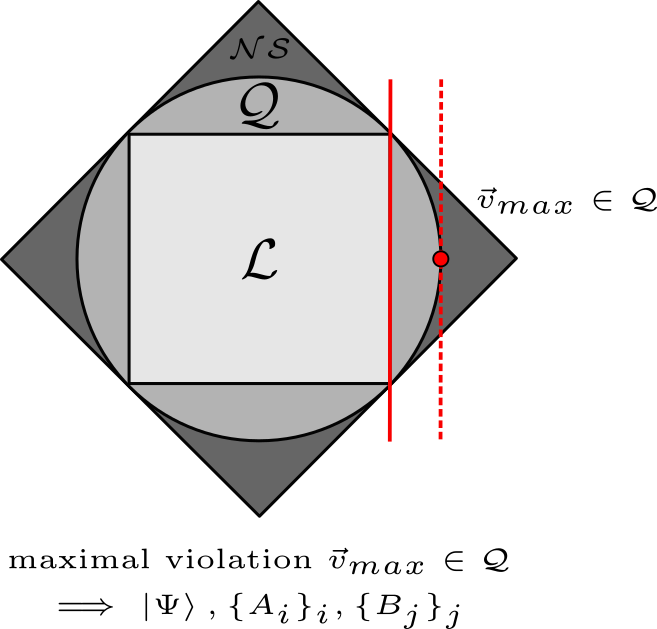
\includegraphics[width=0.6\textwidth]{images/self-testingcorr.png}
    \caption{Schematic drawing depicting the geometry of the convex sets $\mathcal{L}$, $\mathcal{Q}$, and $\mathcal{NS}$, containing all local, quantum, and no-signalling correlations, respectively. A Bell inequality, like the CHSH inequality, defines a separative hyperplane such that all local correlations $\mathcal{L}$ lie to one ``side" of this hyperplane, here represented by the unbroken red line. The extremal point(s) $\Vec{v}_{max}\in\mathcal{Q}$ of the set of quantum correlations $\mathcal{Q}$ corresponds to a maximal violation of the CHSH inequality. The CHSH inequality can be used for self-testing, as the quantum model $\ket{\Psi}$,$\{\Pi_i\}_i$ compatible with a maximal violation of the inequality is unique, up to trivial degrees of freedom.}
    \label{fig:selftestingcorr}
\end{figure}

\begin{figure}
    \centering
    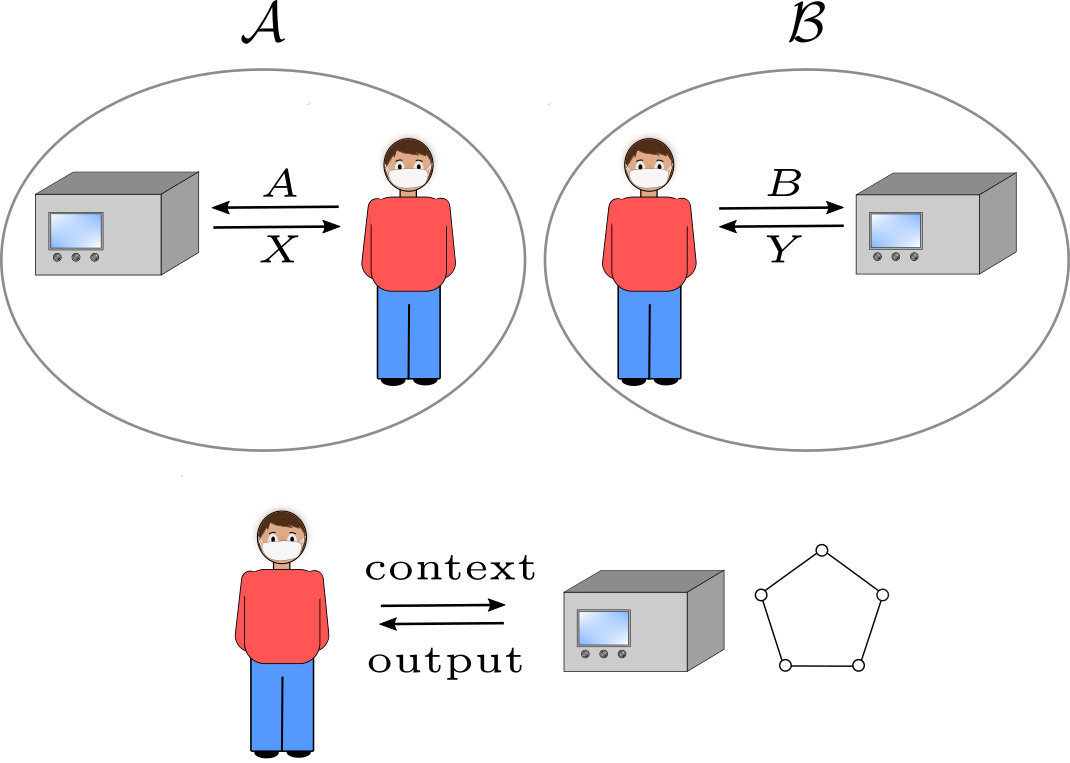
\includegraphics[width=0.8\textwidth]{images/self-testing.png}
    \caption{\textbf{Top}: Typical device-independent Bell-type self-testing scenario. The two subsystems $\mathcal{A}$ and $\mathcal{B}$ are space-like separated. Accordingly, the black box device, which can be interpreted as a correlation experiment testing a Bell inequality, is split into two non-communicating parts. An experimenter can interact classically with a local sub-device, by passing an input value and recording the outcome returned by the device. A violation of the tested Bell inequality implies that the corresponding correlations were obtained by quantum means, i.e.\ joint measurements on an entangled state shared between $\mathcal{A}$, $\mathcal{B}$. For some Bell inequalities, a maximal violation is only compatible with an essentially unique quantum realization, i.e.\ quantum state and set of measurements.
    \textbf{Bottom:} In contrast, self-testing protocols based on KS non-contextuality inequality violations do not assume the device to be split into multiple non-communicating parts. Instead, a single experimenter interacts classically with the device by freely choosing between measurement contexts and determining the corresponding outcome probabilities. Dropping the unnatural assumption of space-like separation complicates the problem of self-testing considerably and we are required to make additional assumptions about the device, for example regarding compatibility relations and information carrying capacity. Thus, contextuality-based self-testing protocols are only semi-device-independent.}
    \label{fig:selftesting}
\end{figure}
